\documentclass[fr]{../../../../../../eplexam}
\usepackage{../../../info-FSAB1402-exam}
\usepackage{../../../../../../eplcode}
\usepackage{listings}

\hypertitle{info-FSAB1402}{3}{FSAB}{1402}{2016}{Janvier}
{Martin Braquet}
{Peter Van Roy}

\section{Programmation fonctionnelle ( /4)}

Suivez les instructions suivantes :

\begin{itemize}

\item  Supposez deux matrices représentées en liste de listes
$$P = [[p_{11} \ldots p_{1b}][p_{21} \ldots p_{2 b}] \ldots [p_{a 1}\ldots p_{ab}]]$$
$$Q = [[q_{11} \ldots q_{1 n}][q_{21} \ldots q_{2 n}]\ldots [q_{m 1} \ldots q_{mn}]]$$
La taille de $P$ est (a x b) et la taille de $Q$ est (m x n). Nous supposons que $a \leq m$ et $b \leq n$.
Les éléments $p_{ij}$ et $q_{ij}$ ont la valeur 0 ou 1. Chaque valeur 1 représente un carré et chaque valeur 0
représente un vide. $P$ représente une figure connexe que l’on appelle un polyomino. $Q$ représente une figure
pas forcément connexe qui contient un certain nombre de carrés répartis dans un rectangle de taille (m x n).

Par exemple :
$$P = [[1\: 0\: 0][1 \:0\: 0][1\: 1\: 1]]$$
$$Q = [[1 \:0 \:0 \:1][0 \:0 \:1 \:0][0\: 1 \:0 \:0]]$$
représente
\begin{figure}[h]
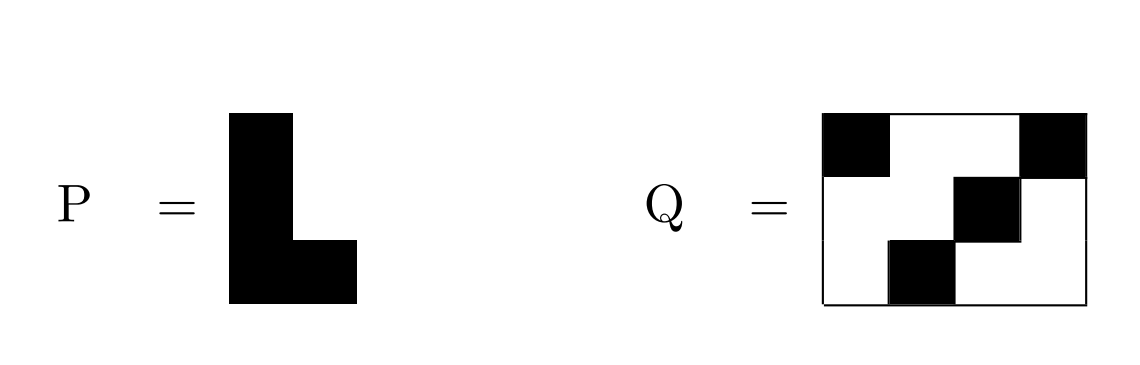
\includegraphics[width=\columnwidth]{PQ.png}
\end{figure}

\item Définissez la fonction \lstinline|{Match P Q}| qui renvoie \lstinline|yes| si $P$ peut se caser dans le coin supérieur gauche de $Q$
et \lstinline|no| sinon. C’est à dire, pour chaque élément $p_{ij}$ de $P$ qui est 1, l’élément correspondant de $Q$ est 0.
Pour les deux figures illustrées ci-dessus, \lstinline|{Match P Q}| = \lstinline|no|.
\item Définissez la fonction \lstinline|{Find P Q}| qui renvoie \lstinline|found(i j)| si P peut se caser quelque part dans Q et le coin
supérieur gauche de $P$ se trouve à la rangée $i$ et la colonne $j$ de $Q$. S’il n’y a pas de possibilités de caser $P$
complètement à l’intérieur du rectangle $Q$, alors la fonction renvoie \lstinline|notfound|.

\end{itemize}

Définissez \lstinline|Match| et \lstinline|Find| en utilisant uniquement des fonctions récursives terminales et déclaratives. Attention à utiliser une fonction par boucle. C’est à dire, pour traverser toutes les cases de $P$ ( ou de $Q$) il faut deux
fonctions récursives terminales. Attention à donner une spécification pour chaque fonction auxiliaire que vous
définissez.

\begin{solution}

\lstinputlisting{Janvier-2016-Q1.oz}

\end{solution}

\section{Sémantique ( /5))}
Voici un petit programme:

\lstinputlisting{Q2.oz}

Répondez aux question suivantes:
\begin{itemize} 

	\item Qu'est-ce qui est affiché quand on exécute ce programme ? ( /0,5)
 
	\item Donnez la traduction de ce programme en langage noyau. Attention à donner une traduction complète ! ( /1)
 
	\item Donnez les environnements contextuels des procédures dans cette traduction. ( /0,5)
 
	\item Donnez quelques pas d'exécution de la machine abstraite pour bien montrer les choses suivantes: 
 
 \begin{itemize}
 \item La création ( /0,5) et l'affectation ( /1) d'une cellule. 

	\item La définition ( /0,5) et l'appel ( /1) d'une procédure. 
 \end{itemize}
	
\end{itemize} 

Attention à ne pas faire plus d'un pas d'exécution dans la machine abstraite pour chacun des 4 cas demandés.

\begin{solution}

\begin{itemize}
    \item Il affiche 2.
    \item \lstinputlisting{Q2(sol).oz}
    \item $$CE_F=\{C\rightarrow c\}$$
    $$CE_{R3}=\{C\rightarrow c,A\rightarrow i7\}$$
    $$CE_{P1}=\{C\rightarrow c\}$$
    \item
Toute l'exécution de la machine abstraite est effectuée. Les états d'exécution à fournir à l'examen sont signalés ci-dessous.

\begin{enumerate}
    \item 
    $$ \Big([(<l1-l26>,\emptyset)],\emptyset,\emptyset\Big) $$
    \item Avant la création d'une cellule
    $$ \Big([(<l2-l25>,E_1=\{C\rightarrow c ,F\rightarrow f,P1\rightarrow p1,R3,\rightarrow r3,R4\rightarrow r4,A1\rightarrow a1,$$
    $$I7\rightarrow i7,Browse \rightarrow browse,NewCell\rightarrow newcell\})],\sigma_2=\{c,f,p1,r3,r4,a1,i7,$$
    $$newcell=(proc\{\$ \:X\: Y\} \ldots end,CE_{Newcell}),browse=(proc\{\$\: X\}\ldots end,CE_{Browse})\},\emptyset\Big) $$
    \item Après la création d'une cellule
    $$ \Big([(<l3-l25>,E_1)],\sigma_2\cup\{a1=0,c=\xi\},\{c:a1\}\Big) $$
    \item 
    $$ \Big([(<l23-l25>,E_1)],\sigma_3\cup\{f=(proc\{\$\: A\:R\}<l4-l11>end,CE_{F}=\{C\rightarrow c\}),$$
    $$p1=(proc\{\$\: R5\}<l14-l21>end,CE_{P1}=\{C\rightarrow c\})\},\{c:a1\}\Big) $$
    \item Avant la définition d'une procédure
    $$ \Big([(<l4-l11>,\{C\rightarrow c, A\rightarrow i7, R\rightarrow r3\}),(<l24-l25>,E_1)],\sigma_4,\{c:a1\}\Big) $$
    \item Après la définition d'une procédure
    $$ \Big([(<l24-l25>,E_1)],$$
    $$\sigma_4\cup\{r3=(proc\{\$\: B\:R2\}<l5-l10>end,CE_{R3}=\{C\rightarrow c,A\rightarrow i7\})\},\{c:a1\}\Big) $$
    \item 
    $$ \Big([(<l5-l10>,\{ C\rightarrow c,A\rightarrow i7,B\rightarrow p1,R2\rightarrow r4 \}),(<l25>,E_1)],\sigma_6,\{c:a1\}\Big) $$
    \item 
    $$ \Big([(<l6-l9>,E_3=\{ C\rightarrow c,A\rightarrow i7,B\rightarrow p1,R2\rightarrow r4,I1\rightarrow i1,I2\rightarrow i2,I3\rightarrow i3 \}),$$
    $$(<l25>,E_1)],\sigma_6\cup\{i1,i2,i3\},\{c:a1\}\Big) $$
    \item 
    $$ \Big([(<l7-l9>,E_3),(<l25>,E_1)],\sigma_8\cup\{i1=0\},\{c:a1\}\Big) $$
    \item 
    $$ \Big([(<l8-l9>,E_3),(<l25>,E_1)],\sigma_9\cup\{i2=1\},\{c:a1\}\Big) $$
    \item Avant l'appel d'une procédure
    $$ \Big([(<l8>,E_3),(<l9>,E_3),(<l25>,E_1)],\sigma_{10},\{c:a1\}\Big) $$
    \item Après l'appel d'une procédure
    $$ \Big([(<l14-l21>,\{ C\rightarrow c, R5\rightarrow i3 \}),(<l9>,E_3),(<l25>,E_1)],\sigma_{11},\{c:a1\}\Big) $$
    \item 
    $$ \Big([(<l15-l20>,E_4=\{ C\rightarrow c, R5\rightarrow i3, I4\rightarrow i4,I5\rightarrow i5, I6\rightarrow i6\}),$$
    $$(<l9>,E_3),(<l25>,E_1)],\sigma_{12}\cup\{i4,i5,i6\},\{c:a1\}\Big) $$
    \item 
    $$ \Big([(<l15>,E_4),(<l16-l20>,E_4),
    (<l9>,E_3),(<l25>,E_1)],\sigma_{13},\{c:a1\}\Big) $$
    \item 
    $$ \Big([(<l16-l20>,E_4), (<l9>,E_3),(<l25>,E_1)],\sigma_{14}\cup\{i4=0\},\{c:a1\}\Big) $$
    \item Avant l'affectation d'une cellule
    $$ \Big([(<l19>,E_4),(<l20>,E_4), (<l9>,E_3),(<l25>,E_1)],$$
    $$\sigma_{15}\cup\{i5=1,i6=1\},\{c:a1\}\Big) $$
    \item Après l'affectation d'une cellule
    $$ \Big([(<l20>,E_4),(<l9>,E_3),(<l25>,E_1)],\sigma_{16},\{c:i6\}\Big) $$
    \item 
    $$ \Big([(<l9>,E_3),(<l25>,E_1)],\sigma_{17}\cup\{i3=1\},\{c:i6\}\Big) $$
    \item 
    $$ \Big([(<l25>,E_1)],\sigma_{18}\cup\{r4=2\},\{c:i6\}\Big) $$
    \item Affiche 2.
    $$ \Big([],\sigma_{20}=\{newcell=(proc\{\$ \:X\: Y\}\ldots end,CE_{Newcell}),$$
    $$browse=(proc\{\$\: X\}\ldots end,CE_{Browse}),a1=0,c=\xi,$$
    $$f=(proc\{\$\: A\:R\}<l4-l11>end,CE_{F}=\{C\rightarrow c\}),$$
    $$ p1=(proc\{\$\:R5\}<l14-l21>end,CE_{P1}=\{C\rightarrow c\}),$$
    $$r3=(proc\{\$\:B\:R2\}<l5-l10>end,CE_{R3}=\{C\rightarrow c,A\rightarrow i7\}), i1=0,$$
    $$i2=1,i4=0,i5=1,i6=1,i3=1,r4=2\},\{c:i6\}\Big) $$
    
    
\end{enumerate}

La pile d'instuctions est vide, le programme est terminé.

\end{itemize}

\end{solution}

\section{Vocabulaire ( /4)}

Définir :

\begin{itemize}

\item Environnement contextuel d’une procédure (avec exemple en fragment de code)
\item Définitions formelles (mathématiques) de la notation grand $O$ et la notation grand $\Omega$
\item Type abstrait (une forme d’abstraction de données) (avec exemple en fragment de code)
\item Sémantique des instructions try et raise (diagramme complet comme vu dans le cours)

\end{itemize}

\end{document}

